%%%%%%%%%%%%%%%%%%%%%%%%%%%%%%%%%%%%%%%%%%%%%%%%%%%%%%%%%%%%%%%%%%%%%%%%%%%%
%% Author template for Marketing Science (mksc)
%% Mirko Janc, Ph.D., INFORMS, mirko.janc@informs.org
%% ver. 0.95, December 2010
%%%%%%%%%%%%%%%%%%%%%%%%%%%%%%%%%%%%%%%%%%%%%%%%%%%%%%%%%%%%%%%%%%%%%%%%%%%%
\documentclass[mnsc,nonblindrev]{informs3} % current default for manuscript submission
% \documentclass[mksc,nonblindrev]{informs3}

\usepackage[hidelinks]{hyperref}
\usepackage{float}

\usepackage[nameinlink,capitalize]{cleveref}
\newcommand{\pb}{p^{PB*}}
\newcommand{\ts}{\tilde{\sigma}}
\newcommand{\pts}{\frac{\partial\pb}{\partial\ts}}

%%\OneAndAHalfSpacedXI % current default line spacing
\OneAndAHalfSpacedXII
%%\DoubleSpacedXII
%%\DoubleSpacedXI

% If hyperref is used, dvi-to-ps driver of choice must be declared as
%   an additional option to the \documentclass. For example
%\documentclass[dvips,mksc]{informs3}      % if dvips is used
%\documentclass[dvipsone,mksc]{informs3}   % if dvipsone is used, etc.

% Private macros here (check that there is no clash with the style)

% Natbib setup for author-year style
\usepackage{natbib}
 \bibpunct[, ]{(}{)}{,}{a}{}{,}%
 \def\bibfont{\small}%
 \def\bibsep{\smallskipamount}%
 \def\bibhang{24pt}%
 \def\newblock{\ }%
 \def\BIBand{and}%

%% Setup of theorem styles. Outcomment only one. 
%% Preferred default is the first option.
\TheoremsNumberedThrough     % Preferred (Theorem 1, Lemma 1, Theorem 2)
%\TheoremsNumberedByChapter  % (Theorem 1.1, Lema 1.1, Theorem 1.2)

%% Setup of the equation numbering system. Outcomment only one.
%% Preferred default is the first option.
\EquationsNumberedThrough    % Default: (1), (2), ...
%\EquationsNumberedBySection % (1.1), (1.2), ...

% In the reviewing and copyediting stage enter the manuscript number.
%\MANUSCRIPTNO{} % When the article is logged in and DOI assigned to it,
                 %   this manuscript number is no longer necessary

%%%%%%%%%%%%%%%%
\begin{document}
%%%%%%%%%%%%%%%%

% Outcomment only when entries are known. Otherwise leave as is and 
%   default values will be used.
%\setcounter{page}{1}
%\VOLUME{00}%
%\NO{0}%
%\MONTH{Xxxxx}% (month or a similar seasonal id)
%\YEAR{0000}% e.g., 2005
%\FIRSTPAGE{000}%
%\LASTPAGE{000}%
%\SHORTYEAR{00}% shortened year (two-digit)
%\ISSUE{0000} %
%\LONGFIRSTPAGE{0001} %
%\DOI{10.1287/xxxx.0000.0000}%

% Author's names for the running heads
% Sample depending on the number of authors;
% \RUNAUTHOR{Jones}
% \RUNAUTHOR{Jones and Wilson}
% \RUNAUTHOR{Jones, Miller, and Wilson}
% \RUNAUTHOR{Jones et al.} % for four or more authors
% Enter authors following the given pattern:
%\RUNAUTHOR{}

% Title or shortened title suitable for running heads. Sample:
% \RUNTITLE{Bundling Information Goods of Decreasing Value}
% Enter the (shortened) title:
%\RUNTITLE{}

% Full title. Sample:
% \TITLE{Bundling Information Goods of Decreasing Value}
% Enter the full title:
\TITLE{PetFinder: Predicting Adoption Speed of Pets}

% Block of authors and their affiliations starts here:
% NOTE: Authors with same affiliation, if the order of authors allows, 
%   should be entered in ONE field, separated by a comma. 
%   \EMAIL field can be repeated if more than one author
% \ARTICLEAUTHORS{%
% \AUTHOR{Author1}
% \AFF{Author1 affiliation, \EMAIL{}, \URL{}}
% \AUTHOR{Author2}
% \AFF{Author2 affiliation, \EMAIL{}, \URL{}}
% % Enter all authors
% } % end of the block

\ARTICLEAUTHORS{%
\AUTHOR{Jinyi Liu}
\AFF{Haslam College of Business, University of Tennessee, Knoxville, \EMAIL{jinyi.liu@utk.edu}, \URL{https://orcid.org/0009-0009-8600-9965}}
} % end of the block

\ABSTRACT{
In this project, we use Xgboost to predict the adoption speed of pets. We do a feature engineering and use a Xgboost regressor to train the model. This gives us an average of $\kappa=0.4694$ with a standard error $0.01058$ for a 5-fold crossvalidation.
}

% Sample
%\KEYWORDS{deterministic inventory theory; infinite linear programming duality; 
%  existence of optimal policies; semi-Markov decision process; cyclic schedule}

% Fill in data.
\KEYWORDS{Classification, Supervised Learning, Xgboost, Feature Engineering}

\maketitle
%%%%%%%%%%%%%%%%%%%%%%%%%%%%%%%%%%%%%%%%%%%%%%%%%%%%%%%%%%%%%%%%%%%%%%

% Samples of sectioning (and labeling) in MKSC
% NOTE: (1) \section and \subsection do NOT end with a period
%       (2) \subsubsection and lower need end punctuation
%       (3) capitalization is as shown (title style).
%
%\section{Introduction.}\label{intro} %%1.
%\subsection{Duality and the Classical EOQ Problem.}\label{class-EOQ} %% 1.1.
%\subsection{Outline.}\label{outline1} %% 1.2.
%\subsubsection{Cyclic Schedules for the General Deterministic SMDP.}
%  \label{cyclic-schedules} %% 1.2.1
%\section{Problem Description.}\label{problemdescription} %% 2.

% Text of your paper here

\section{Background and Motivation}\label{Background} 
Millions of stray animals suffer on the streets or are euthanized in shelters every day around the world. If homes can be found for them, many precious lives can be saved --- and more happy families created. 

PetFinder.my has been Malaysia's leading animal welfare platform since 2008, with a database of more than 150,000 animals. PetFinder collaborates closely with animal lovers, media, corporations, and global organizations to improve animal welfare.

In this project, we use PetFinder.my's database to create an algorithm that predicts how quickly a pet will be adopted. From this, PetFinder can improve their pet's profile to attract more potential adopters. 

% \subsection{Objectives}


% Clearly state your objective. 

% Provide a problem formulation. 

% Justify your choice of model(s).

% For this mid-term assessment, you only need to demonstrate your ability of abstracting an application problem into a technical formuation. What is given, what do you look for, and what are the constraints or considerations (if applicable)?

% Hint: By working on this assignment, you should have tools for feature preparation, supervised learning, and unsupervised learning for insights.
% Design your experiments and show your point. E.g.,
% How do you ensure that your model is properly fit?
% If not using your current approach, what would be the alternative approaches?
% How do you evaluate the models?
% Did you tune the hyperparameters?
% For an applied paper, it is important to (1) show that your model worked the best you can; (2) discuss the practical implications. 
\section{Problem Statement}

\subsection{Data}
The training data set consists of 14993 pet profiles. Each profile contains the following features: 
\begin{itemize}
    \item \textbf{AdoptionSpeed} - Categorical speed of adoption. Lower is faster. \textbf{This is the value to predict.}
    \item \textbf{PetID} - Unique hash ID of pet profile
    \item \textbf{Type} - Type of animal 
    \item \textbf{Name} - Name of pet 
    \item \textbf{Age} - Age of pet when listed, in months
    \item \textbf{Breed1, Breed2} - Breeds of pet 
    \item \textbf{Gender} - Gender of pet 
    \item \textbf{{Color1, Color2, Color3}} - Colors of pet 
    \item \textbf{MaturitySize} - Size at maturity 
    \item \textbf{FurLength} - Fur length 
    \item \textbf{Vaccinated} - Pet has been vaccinated
    \item \textbf{Dewormed} - Pet has been dewormed 
    \item \textbf{Sterilized} - Pet has been spayed / neutered 
    \item \textbf{Health} - Health Condition 
    \item \textbf{Quantity} - Number of pets represented in profile
    \item \textbf{Fee} - Adoption fee 
    \item \textbf{State} - State location in Malaysia 
    \item \textbf{RescuerID} - Unique hash ID of rescuer
    \item \textbf{VideoAmt} - Total uploaded videos for this pet
    \item \textbf{PhotoAmt} - Total uploaded photos for this pet
    % \item \textbf{Description} - Profile write-up for this pet. The primary language used is English, with some in Malay or Chinese.
\end{itemize}

\subsection{Aim}
Animal adoption rates are strongly correlated to the metadata associated with their online profiles. In this project, we use this dataset to create an algorithm that predicts how quickly a pet will be adopted. The adoption speed is determined by how quickly, if at all, a pet is adopted. The values are determined in the following way:
\begin{enumerate}
    \item[0 --]  Pet was adopted on the same day as it was listed.
    \item[1 --]  Pet was adopted between 1 and 7 days (1st week) after being listed.
    \item[2 --]  Pet was adopted between 8 and 30 days (1st month) after being listed.
    \item[3 --] Pet was adopted between 31 and 90 days (2nd \& 3rd month) after being listed.
    \item[4 --] No adoption after 100 days of being listed. (There are no pets in this dataset that waited between 90 and 100 days).
\end{enumerate}

\subsection{Model}
Since the adoption speed to be predicted is categorical, we adopt a xgboost model. This model is a gradient boosting algorithm that is optimized for speed and performance. It is based on decision trees and is a popular choice for machine learning competitions.

\subsection{Evaluation}
We use quadratic weighted kappa to evaluate the performance of our model. Predicted results have 5 possible ratings, $0,1,2,3,4$. The quadratic weighted kappa is calculated as follows. First, an $\mathrm{N} \times \mathrm{N}$ histogram matrix $O$ is constructed, such that $O_{i, j}$ corresponds to the number of adoption records that have a rating of $i$ (actual) and received a predicted rating j. An $\mathrm{N}\times \mathrm{N}$ matrix of weights, $w$, is calculated based on the difference between actual and predicted rating scores:
$$
w_{i, j}=\frac{(i-j)^2}{(N-1)^2}
$$
An $\mathrm{N}\times \mathrm{N}$ histogram matrix of expected ratings, $E$, is calculated, assuming that there is no correlation between rating scores. This is calculated as the outer product between the actual rating's histogram vector of ratings and the predicted rating's histogram vector of ratings, normalized such that $E$ and $O$ have the same sum.
From these three matrices, the quadratic weighted kappa is calculated as:
$$
\kappa=1-\frac{\sum_{i, j} w_{i, j} O_{i, j}}{\sum_{i, j} w_{i, j} E_{i, j}}.
$$  
The metric $\kappa$ typically varies in $[0,1]$. The higher the $\kappa$, the better the agreement between the raters. A value of $0$ indicates agreement equivalent to chance, and a value of $1$ indicates perfect agreement. In the event that there is less agreement between the raters than expected by chance, $\kappa$ can be negative.
\section{Experiment and Results}
There are 14993 pet profiles in the training data set and contains 23 features. 
\subsection{Data Preprocessing}
Since we adopt the Xgboost method, the missing value is not a problem. We combine the breed and color features into one feature. For example, if the pet has two breeds, we combine the two breeds into one feature. If the pet has three colors, we combine the three colors into one feature. We also add one more column named hard-interaction which conbines pet's type, gender, vaccinated, dewormed and sterilized status. Some profiles contain multiple pets so we calculate the average fees and photos to create a new column. Furthermore, there are some pets without a name, we think this matters for the adoption speed so we add one more column to indicate whether the pet has a name and also the name length and strangeness of the name.\footnote{We assume the name is strange if it contains number and special characters.} The breed of the pet is also an important factor. Thus, we add features to consider the breed name, breed number, mixed breed, domestic breed and whether it's pure. 

\subsection{Feature Engineering}
To better train the model, we do a feature engineering. We briefly introduce the features we add in this section and leave the details in the appendix code. We add the following features:
Color, Breed, State, State-Breed1-Color1, State-BreedFull-ColorFull, Name, RescuerID, Hard-Interaction. For each one, we calculate the mean, minimum, maximum and standard deviation. After that we drop the mentioned features and only keep the new features since they are highly correlated. After this, we get a new 136 numerical features. 

\subsection{Model}
\subsubsection{Xgboost Classifier}
Intuitively, we think the Xgboost classifier is a good choice for this problem since the predicted variable has 5 values. We use the Xgboost classifier to train the model. To find the best hyperparameters, we do a grid search and find the best hyperparameters.\footnote{It costs us 4 hours. The hyperparameters are shown in the appendix for brevity.} This model gives us an average of $\kappa=0.40$ which is not good enough. 

\subsubsection{Xgboost Regressor}
Since the Xgboost classifier does not give us a good result, we try the Xgboost regressor. We do a new grid search for the best hyperparameters. In this case, we choose the best hyperparameters as follows:
\begin{itemize}
    \item objective: reg:squarederror
    \item eval\_metric: rmse
    \item max\_depth: 7
    \item subsample: 0.8
    \item colsample\_bytree: 0.8
    \item $\alpha$: 0.05
    \item $\eta$: 0.01
\end{itemize}
To be clear, since we use a regression model, the predicted value is not an integer. We use the following method to convert the predicted value to an integer:
\begin{enumerate}
    \item Calculate the c.d.f. of the AdoptionSpeed in the training set and store the result in a list $c=[c_0,c_1,c_2,c_3]$. 
    \item Predict the values for the training set and have the minimum $p_{\min}$ and the gap between maximum and minimum as $\delta$. We then have the cutoff value as cutoff values$=p_{\min}+\delta c=[d_0,d_1,d_2,d_3]$.
    \item Predict the values for the validation set, and for each value $v$, we find the smallest $i$ such that $v\leq d_i$. Then we set the predicted value as $i$. If no such $i$ exists, we set the predicted value as $4$.
\end{enumerate}
This gives us an average of $\kappa=0.4694$ with a standard error $0.01058$ for a 5-fold crossvalidation, which is better than the Xgboost classifier.  


\section{Discussion and Implications}
We do not use the image and the metadata in this project. We think the image and the metadata are important for the adoption speed. However, we do not have enough time to do the image analysis and the metadata analysis. We think the image analysis is a good direction for future research. Also, there is also a lot of information in the description of the pet. We think the description is also a good direction for future research. Though we don't use the image and the metadata, we think the result is good enough. A $\kappa$ of $0.4694$ is not bad since we only use 176 features to predict the adoption speed. 
\begin{figure}[H]
    \centering
    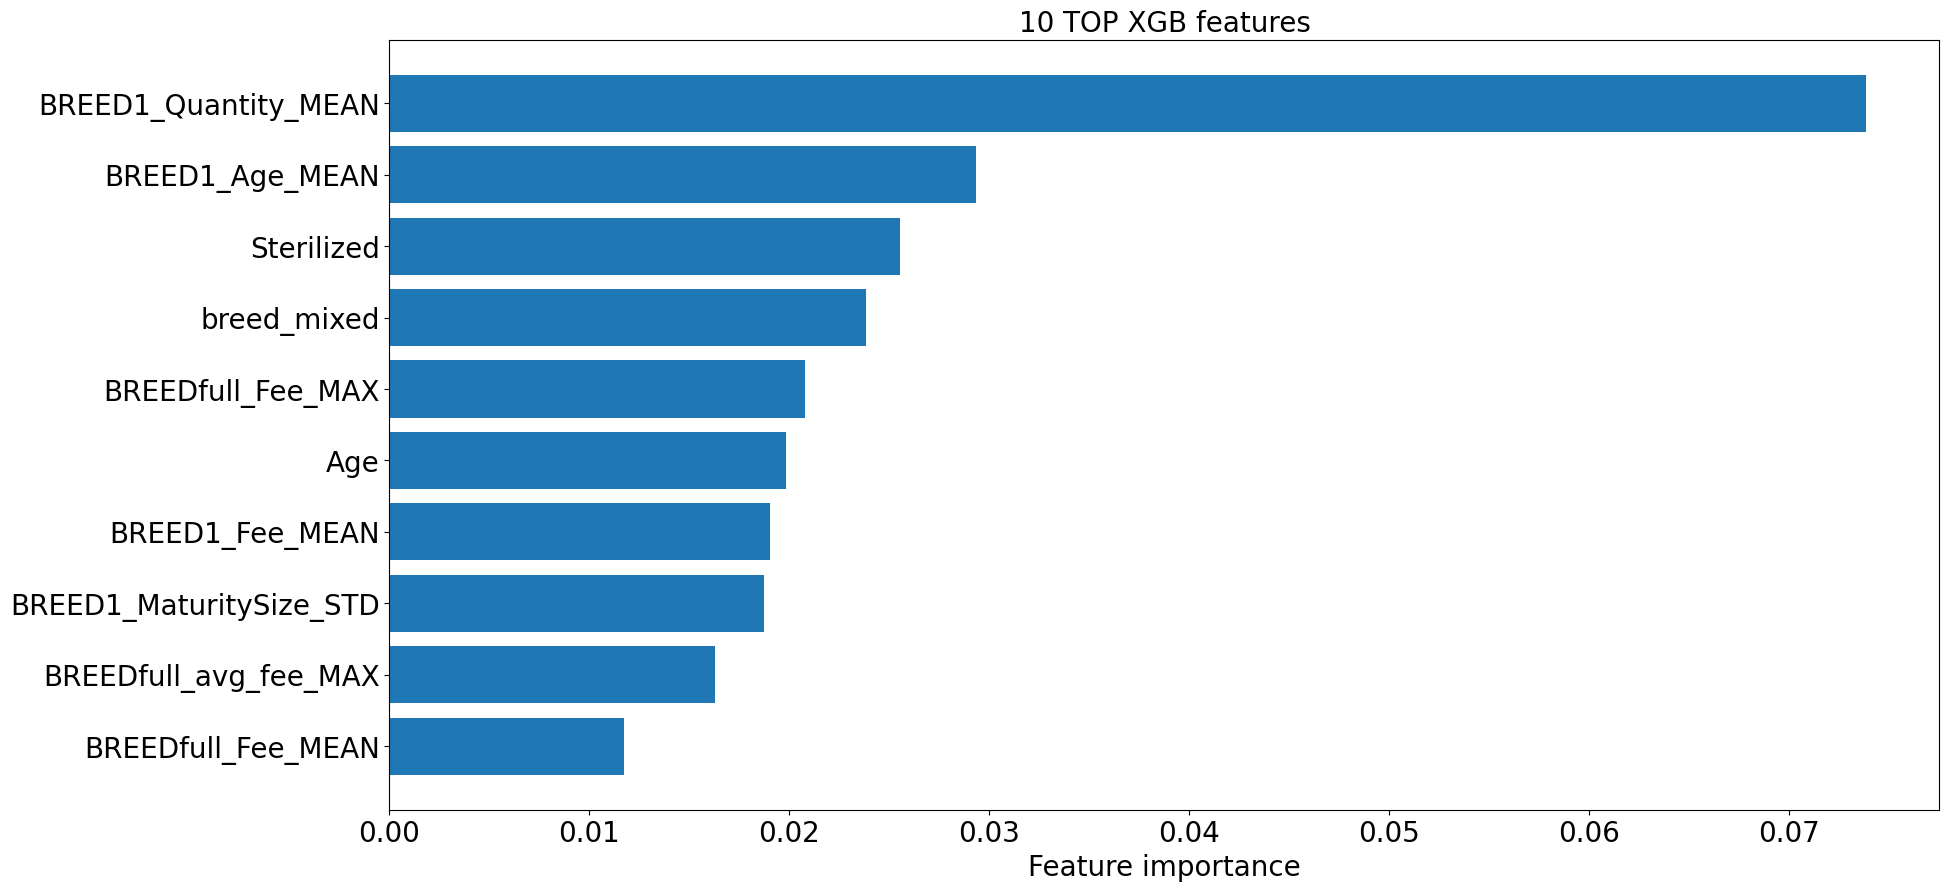
\includegraphics[width=1\textwidth]{code/figure/xgb_feature_importance.png}
    \caption{Feature importance}
    \label{fig:feature_importance}
\end{figure}
From \Cref{fig:feature_importance} we can see that, the main breed, i.e., Breed1, is the most important factor affecting the adoption speed. Also, whether is sterilized, whether is breed is mixed and the age of the pets are also important factors. This is intuitive since in reality, people tend to adopt pets with a younger age. Also, the sterilized status is also important since people tend to adopt pets that are sterilized. The color of the pet is not important. This is reasonable since the color of the pet is not a good indicator of the adoption speed. We can also see that, the adoption fee also matters. 

Thus, to improve the adoption speed, we can do the following things:
\begin{itemize}
    \item Highlight the main breed of the pet.
    \item Show mixed breed.
    \item Sterilize the pet.
    \item Highlight the age of the pet.
    \item Set a reasonable adoption fee.
\end{itemize}


% Acknowledgments here
% \ACKNOWLEDGMENT{%
% % Enter the text of acknowledgments here
% }% Leave this (end of acknowledgment)

\begin{APPENDIX}{}
The code and the data is available at \url{https://github.com/Jinyi-Liu/BZAN645-Midterm}.
\end{APPENDIX}
%
\section{Declarations}
All authors certify that they have no affiliations with or involvement in any organization or entity with any financial interest or non-financial interest in the subject matter or materials discussed in this manuscript. The authors have no funding to report.


% \textbf{Declarations}: \textit{All authors certify that they have no affiliations with or involvement in any organization or entity with any financial interest or non-financial interest in the subject matter or materials discussed in this manuscript. The authors have no funding to report.}


% References here (outcomment the appropriate case) 

% CASE 1: BiBTeX used to constantly update the references 
%   (while the paper is being written).
\bibliographystyle{informs2014} % outcomment this and next line in Case 1
\bibliography{refer.bib} % if more than one, comma separated

% CASE 2: BiBTeX used to generate mypaper.bbl (to be further fine tuned)
%\input{mypaper.bbl} % outcomment this line in Case 2

\end{document}


